%! program = pdflatex

%\documentclass[12pt,a4paper]{memoir} % for a long document
%\documentclass[12pt,a4paper,article]{memoir} % for a short document
\documentclass[12pt,a4paper,article]{memoir}
\usepackage{geometry}
 \geometry{
 a4paper,
 left=20mm,
 right=20mm,
 top=20mm,
 bottom=20mm,
 }
% \usepackage[titletoc]{appendix}

\usepackage{graphicx}
\usepackage{listings}
\usepackage[dvipsnames]{xcolor}
\usepackage{hyperref}
\usepackage{cleveref}

%\lstset{frame=tb,
%  language=C++,
%  aboveskip=3mm,
%  belowskip=3mm,
%  showstringspaces=false,
%  columns=flexible,
%  basicstyle={\small\ttfamily},
%  numbers=none,
%  numberstyle=\tiny\color{mygray},
%  keywordstyle=\color{blue},
%  commentstyle=\color{mygreen},
%  stringstyle=\color{mymauve},
%  breaklines=true,
%  breakatwhitespace=true,
%  tabsize=2
%}

\definecolor{codegreen}{rgb}{0,0.6,0}
\definecolor{codegray}{rgb}{0.5,0.5,0.5}
\definecolor{codepurple}{rgb}{0.58,0,0.82}
\definecolor{backcolour}{rgb}{0.95,0.95,0.92}
 

\lstdefinestyle{MyCodeStyle} {
%  language=C++, % choose the language of the code
  backgroundcolor=\color{backcolour},
  commentstyle=\color{codegreen},
  keywordstyle=\color{magenta},
  numberstyle=\tiny\color{codegray},
  stringstyle=\color{codepurple},
  basicstyle=\footnotesize,
  breakatwhitespace=false,
  breaklines=true,
  captionpos=b, % sets the caption-position to bottom
  keepspaces=true,                 
  numbers=none, % where to put the line-numbers
  showspaces=false, % show spaces adding particular underscores
  showstringspaces=false, % underline spaces within strings
  showtabs=false, % show tabs within strings adding particular underscores
  frame=single, % adds a frame around the code
  tabsize=2, % sets default tabsize to 2 spaces
  rulesepcolor=\color{blue},
  rulecolor=\color{black},
  xleftmargin=.1\textwidth,
  xrightmargin=.1\textwidth,
}

\hypersetup{
    colorlinks,
    citecolor=black,
    filecolor=black,
    linkcolor=black,
    urlcolor=black
}

\graphicspath{ {./img/} }
% See the ``Memoir customise'' template for some common customisations
% Don't forget to read the Memoir manual: memman.pdf

\title{Optimizing Alya simulations of multi-physics problems with Dakota}
\author{Rogeli Grima}
%\date{10/12/2014} % Delete this line to display the current date

% Make appear "Appendix" in the ToC
\renewcommand*{\cftappendixname}{Appendix\space}

%%% BEGIN DOCUMENT
\begin{document}

\maketitle
\tableofcontents*

\chapter{Introduction}

Dakota is a toolkit that provides a flexible, extensible interface between analysis codes and iterative systems analysis methods. It contains algorithms for optimization, uncertainty quantification, parameter estimation and sensitivity/variance analysis.

Alya is a computational method that is used to simulate complex physical systems. On many occasions we want to use these simulations to find an acceptable or optimized solution for a particular system. Dakota will help us to use Alya as a design tool. It will help us to solve very important questions as: What is the best design? How safe is it? How much confidence do I have in my answer?

This user's guide is intended to provide some background information on how to use Dakota to solve optimization problems that involve a simulation with Alya. We assume the user has some familiarity with Alya execution and configuration.

In this guide we will show how to use Dakota in Marenostrum, how to prepare your simulations with Alya, how to process their outputs and we will provide some basic examples.

\section{Dakota workflow}

Before you start working with Dakota and Alya, is important to know the Dakota's workflow. This will give you a better perspective of what is happening.

Dakota receives input and configuration from a variety of text files prepared by the user, and connects to any simulation code by other text files. This simple interface is one of the most important features of Dakota, as it makes it easy to change the iterative method or strategy by just changing a few lines in the Dakota input file.

In Figure \ref{fig:Workflow}, we can see the Dakota workflow. The user should provide an input file to Dakota. This input file controls the algorithm that we want to run, the function to be evaluated, the variables of this function and the outputs that we expect.

\begin{figure}[htb!]
  \centering
    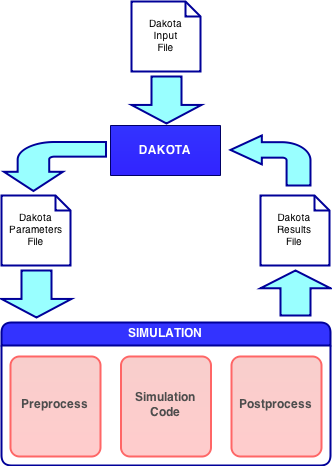
\includegraphics[width=0.4\textwidth]{DakotaWorkflow}
  \caption{Dakota Workflow}
  \label{fig:Workflow}
\end{figure}

Dakota generates a parameter file for every function evaluation. This file contains a specific value of every variable and specifies the kind of returning values that it needs (function evaluation, derivatives or/and second derivatives).

Dakota treats the simulation code as a black box. Most of the codes, like Alya, don't know what to do with the parameter file, so it is common to create a script to connect the simulation code with Dakota. In this script we merge the Dakota parameters file with the simulation code input files. Once we have some proper input files we can run the simulation code, extract the significant data from its output files and post-process that data in order to generate the appropriate objective function and the Dakota results file.

\chapter{Dakota tutorial}
\section{Set up Dakota}

We have installed in Marenostrum the last three versions of Dakota. Althought, most of the experiments that we have ran have been done using version 5.4 we encourage you to use the last version. From now on, all the information that we will provide you in this guide will refer to version 6.1. You can find the several installed versions of Dakota in:

\begin{itemize}
\item \textit{/gpfs/projects/bsc21/DAKOTA/dakota-5.4.0}
\item \textit{/gpfs/projects/bsc21/DAKOTA/dakota-6.0.0}
\item \textit{/gpfs/projects/bsc21/DAKOTA/dakota-6.1.0}
\end{itemize}

If you want to install your own version of Dakota in Marenostrum, please check Appendix \ref{chapter:CodeMod}.


In order to run Dakota you will need to set the path of the executables and the directory of the shared libraries. You can add these lines to your .barshrc file:

\begin{lstlisting}[style=MyCodeStyle,language=bash]
export DAK_INSTALL=/gpfs/projects/bsc21/DAKOTA/dakota-6.1.0
export PATH=${DAK_INSTALL}/bin/:${PATH}
export LD_LIBRARY_PATH=${DAK_INSTALL}/bin:${LD_LIBRARY_PATH}
export LD_LIBRARY_PATH=${DAK_INSTALL}/lib:${LD_LIBRARY_PATH}
\end{lstlisting}

Check that everything is working properly by running:

\begin{lstlisting}[style=MyCodeStyle,language=bash]
dakota -v
\end{lstlisting}

\section{Runing Dakota with a simple input file}
\label{section:RunDakota}

This section is intended for users who are new to Dakota, to demonstrate the basics of running a simple example.

\begin{enumerate}
\item Create a working directory.
\item From path \textit{/gpfs/projects/bsc21/DAKOTA/Examples/power}, copy files \textit{power\_multidim.in} and \textit{power.py} to the working directory.
\item From the working directory, run: \textit{dakota -i power\_multidim.in -o power\_multidim.out \textgreater{} power\_multidim.stdout}
\end{enumerate}

Dakota outputs a large amount of information to help users track progress. Four files should have been created:
\begin{enumerate}
\item The screen output has been redirected to the file power\_multidim.stdout. The contents are messages from Dakota and notes about the progress of the iterator (i.e. method/algorithm).
\item The output file \textit{power\_multidim.out} contains information about the function evaluations.
\item \textit{power\_multidim.dat} is created due to an specification of the input file. This summarizes the variables and responses for each function evaluation.
\item \textit{dakota.rst} is a restart file. If a Dakota analysis is interrupted, it can be often be restarted without losing all progress.
\end{enumerate}

This example used a parameter study method and the \textit{power.py} test problem. The Python script \textit{power.py} reads a Dakota parameters file, computes the function $F(x,y)=(X-0.5)^2+(Y+0.5)^2$ and writes the result in a Dakota results file.

As we said, this is a parametric study. Let's try to execute an optimization problem. Now, copy file \textit{power\_mas.in} to your working directory and run:

%dakota -i  power\_mas.in -o power\_mas.out \textgreater{} power\_mas.stdout
\begin{lstlisting}[style=MyCodeStyle,language=bash]
dakota -i  power_mas.in -o power_mas.out > power_mas.stdout
\end{lstlisting}

This executes a mesh adaptive direct search algorithm. If you look at the output file you will see that the method converges in 160 iterations and propose as a best objective function a value of $F(X,Y)=0.0$ evaluated for $X=0.5$ and $Y=-0.5$ . That is the minimum of the evaluated function.

You can see a graphic representation of the results executing the script \textit{visualize.sh} that you can find in the same directory. This scripts reads the results from the parametric study and from the mesh adaptive direct search algorithm.

\begin{figure}[htb!]
  \centering
    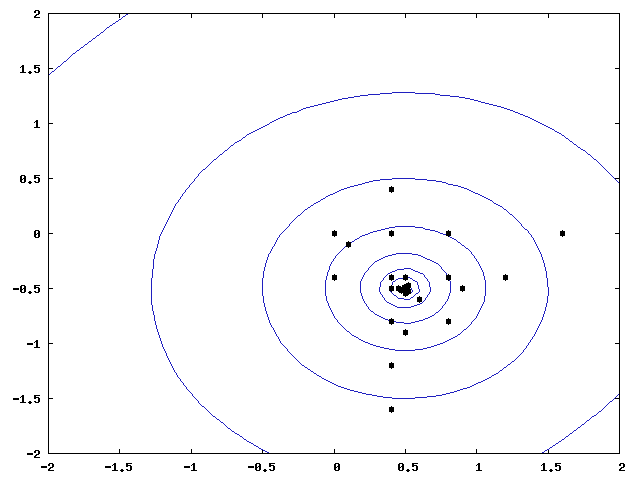
\includegraphics[width=0.5\textwidth]{power}
  \caption{Mesh adaptive direct search evaluation points}
  \label{fig:Power}
\end{figure}

\chapter{Dakota files}

\section{Dakota input file format}

There are six sections in every Dakota input file. These sections are identified with the following keywords: \textit{variables}, \textit{interface}, \textit{responses}, \textit{model}, \textit{method}, and \textit{environment}. At least one \textit{variables}, \textit{interface}, \textit{responses}, and \textit{method} must appear, and no more than one \textit{environment} should appear.

\begin{figure}[htb!]
  \centering
    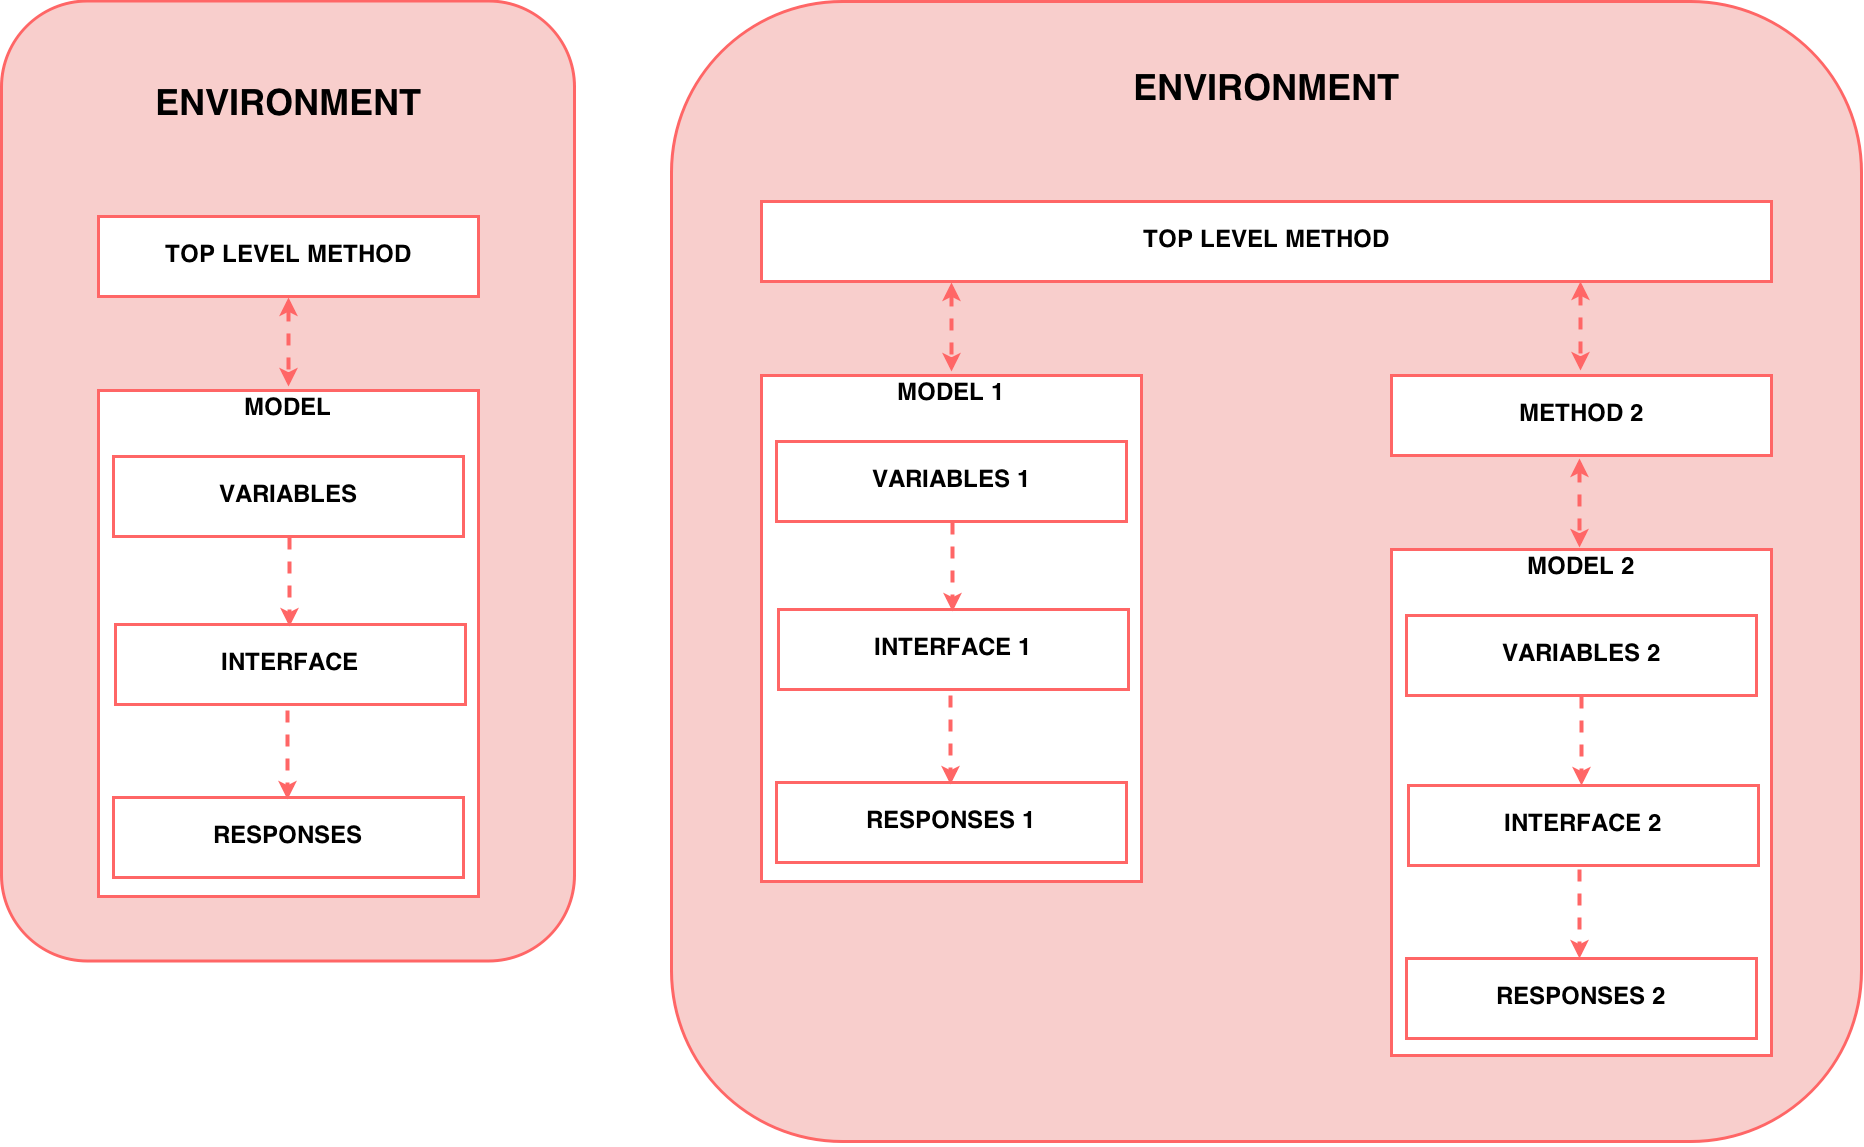
\includegraphics[width=0.8\textwidth]{DakotaInputFile}
  \caption{Relationship between the six blocks}
  \label{fig:InputFile}
\end{figure}

Figure \ref{fig:InputFile} shows the relationships between the six keyword blocks. The environment specifies high level Dakota settings, and identifies the top level method. A method runs a model. A model block defines the connections between variables, the interface, and responses. It shows the most common relationships between blocks but others are possible. Most Dakota analyses just needs to define a single method which runs a single model.

For a more concrete example, a simple Dakota input file, \textit{power\_multidim.in}, for a two-dimensional parameter study on $F(x,y)=(X-0.5)^2+(Y+0.5)^2$ function is shown in Figure \ref{fig:PoMuCode}. This input file will be used to describe the basic format and syntax used in all Dakota input files.

\begin{figure}[htb!]
\begin{lstlisting}[style=MyCodeStyle,language=bash]
environment
  tabular_graphics_data
    tabular_graphics_file = 'power_multidim.dat'

method
  multidim_parameter_study
    partitions = 8 8

model
  single

variables
  continuous_design = 2
    lower_bounds     -2.0     -2.0
    upper_bounds      2.0      2.0
    descriptors       "X"     "Y"

interface
  fork
    analysis_driver = './power.py'
    parameters_file = 'params'
    results_file    = 'results'
    file_save

responses
  response_functions = 1
  no_gradients
  no_hessians
\end{lstlisting}
\caption{File power\_multidim.in}
\label{fig:PoMuCode}
\end{figure}

First, some syntax background:
\begin{itemize}
\item Blocks can follow any order.
\item Comments starts with symbol \textit{\#}.
\item Use of single or double quotes for string inputs.
\item Use of commas and/or white spaces for separation of specifications.
\item The optional use of symbol \textit{=} to indicate supplied data.
\end{itemize}

The first block that we can find in the file is \textit{environment}. This keyword is used to specify the general Dakota settings such as Dakota's graphical output and the tabular data output (via the \textit{tabular\_graphics\_data} keyword).

The \textit{method} block of the input file specifies which iterative method Dakota will employ, such as a parameter study, optimization method, data sampling technique, etc. The keyword \textit{multidim\_parameter\_study} calls for a multidimensional parameter study, while the keyword \textit{partitions} specifies the number of intervals per variable. In this case, there will be eight intervals (nine data points) evaluated between the lower and upper bounds of both variables (bounds provided subsequently in the variables section), for a total of 81 response function evaluations.

The \textit{model} block of the input file specifies the model that Dakota will use. It provides the logical unit for determining how a set of variables is mapped into a set of responses in support of an iterative method. The model allows one to specify a single interface, or to manage more sophisticated mappings involving surrogates or nested iteration. 
Most of the time we are going to use the \textit{single} model, that is the default value for \textit{model} and its definition can be omitted.

The \textit{variables} block of the input file specifies the characteristics of the parameters that will be used in the problem formulation. The variables can be continuous or discrete, and can be classified as design variables, uncertain variables, or state variables. In figure \ref{fig:PoMuCode} you can see as we have defined two continuous design variables, with their upper and lower bounds and a name: X and Y.

The \textit{interface} block of the input file specifies what approach will be used to map variables into responses as well as details on how Dakota will pass data to and from a simulation code. In this example, the keyword \textit{fork} is used to indicate the use of a user-supplied program. Then we find four keywords: 
\begin{itemize}
\item \textit{analysis\_driver:} indicates the name of the program to execute. In this case, it is going to use the python program \textit{power.py}. 
\item \textit{parameters\_file:} name of the dakota parameters file that the driver would receive from Dakota.
\item \textit{results\_file:} name of the results file that the driver should return to Dakota once it has finished.
\item \textit{file\_save:} It's telling Dakota to not delete parameters and results files once the driver has finished.
\end{itemize}

Dakota will execute the external program like this:

\begin{lstlisting}[style=MyCodeStyle,language=bash]
./power.py params.$i results.$i
\end{lstlisting}

Where \$i is the iteration number of the method.

The \textit{responses} block of the input file specifies the types of data that the interface will return to Dakota. For our example, the assignment \textit{num\_objective\_functions = 1} indicates that there is only one objective function. Since there are no constraints associated with Rosenbrock's function, the keywords for constraint specifications are omitted. The keywords \textit{no\_gradients} and \textit{no\_hessians} indicate that no
derivatives will be provided to the method; none are needed for a parameter study.

\section{Dakota parameters file format}

Prior to invoking a simulation, Dakota creates a parameters file which contains the current parameter values and a set of function requests. Let's execute the same example that we ran in section \ref{section:RunDakota}, but first, uncomment the line that contains \textit{file\_save}. This will prevent Dakota to remove the temporal files that it uses to communicate with the simulation program. If you list your working directory you will see 81 parameters files (params.*) and 81 results files (results.*). This is how it looks like the content of file \textit{params.1}:

\begin{lstlisting}[style=MyCodeStyle,language=bash]
                                          2 variables
                     -2.000000000000000e+00 X
                     -2.000000000000000e+00 Y
                                          1 functions
                                          1 ASV_1:response_fn_1
                                          2 derivative_variables
                                          1 DVV_1:X
                                          2 DVV_2:Y
                                          0 analysis_components
                                          1 eval_id
\end{lstlisting}

This file can be interpreted as a sequence blocks, where every block contains an array.
\begin{itemize}
\item First we find information about variables: the number of variables (2) followed by the variable values and names ($X=-2.0$ and $Y=-2.0$).
\item The second block contains information of the functions: number of functions (1) followed by kind of response. This information is coded in \textit{ASV\_i}. It can be value, gradient and/or Hessian.
\item The third block contains information about active variables.
\item Then information about analysis components.
\item Finally we have an id of the current iteration 
\end{itemize}

\section{Dakota results file format}

Once the simulation code has finished it should return the needed information through a results file. This is the file \textit{results.1}: 

\begin{lstlisting}[style=MyCodeStyle,language=bash]
      8.5 f   
\end{lstlisting}

It returns the function evaluation value. For a general case we will find a line for every requested response, a line for every requested gradient and a line for every requested Hessian.

After a simulation, Dakota expects to read a file containing responses reflecting the current parameters and corresponding to the function requests in the active set vector. The response data must be in proper format. If the amount of data in the file does not match the function request vector, Dakota will abort execution with an error message.

The format of the numeric fields may be floating point or scientific notation. In the latter case, acceptable exponent characters are \textit{E} or \textit{e}.

\chapter{Coupling Alya with Dakota}

Alya is not prepared to read a Dakota parameter file, interpret the data and run the simulation. It cannot generate a Dakota results file. In fact, it probably cannot generate the objective function that we want to optimize. That function may be some kind of combination of the Dakota outputs.

So, If we want to connect Alya simulation code with Dakota we must pre-process Alya inputs and post-process its outputs. In Dakota is very usual to use a bash script to do these steps:

\begin{itemize}
\item Pre-process step: Mix simulation program input files with Dakota parameters file.
\item Simulation step: Run the simulation program.
\item Post process step: Read the needed data from outputs of the simulation, compute a cost function and write the result in the appropriate file.
\end{itemize}

\section{Alya input file preprocessing}

When we run an Alya simulation we will find thousands of parameters in the input files. If we want to run an optimization problem, we must choose the design variables. That means, that the value of that variables can be modified and we must mark those variables in order to be used by Dakota.

In order to mark those variables you should use the same descriptor that you have used in the Dakota input file. For instance, let's imagine that you have a velocity field in one of your Alya input files:

\begin{lstlisting}[style=MyCodeStyle,language=bash]
VELOCITY
	5.0 -4.0 0.0
END VELOCITY  
\end{lstlisting}

If you want to use the two first fields of the velocity as design variables, first you have to create a descriptor for these variables in the Dakota input file:

\begin{lstlisting}[style=MyCodeStyle,language=bash]
variables
  continuous_design = 2
    descriptors     'v_x'     'v_y'
\end{lstlisting}

Then you have to create a template file containing the original Alya input data, but modifying those fields. You should write the descriptor between braces:

\begin{lstlisting}[style=MyCodeStyle,language=bash]
VELOCITY
	{v_x} {v_y} 0.0
END VELOCITY
\end{lstlisting}

This file is ready to be processed with \textbf{dprepro}, which comes with the Dakota distribution. It is an application that can read a Dakota parameter file (variable names and values) and a file supplied by the user (our template file) and generate a file that can be used by our simulation code. Usage:

\begin{lstlisting}[style=MyCodeStyle,language=bash]
dprepro parameters_file template_input_file new_input_file
\end{lstlisting}

If you want to try a simple example:
\begin{itemize}
\item Create a working directory.
\item Copy all files from path \textit{/gpfs/projects/bsc21/DAKOTA/Examples/preproc} to your working directory.
\item Execute: \textit{dprepro params veloc.tmp veloc}
\end{itemize}

If your design variables are stored in different Alya files you will have to create a template file and run dprepro for each one.

\section{Set up Alya execution}

Running one Alya instance for a large problem can consume a lot of resources. Running an optimization problem will require to execute Alya many times. It becomes very important to save these resources as much as possible. We encourage you to use restart files for your executions and to define a proper output set up.

Using a good restart file can speed up your simulation. If the state of the simulation begins close to the solution it will be more stable and it will converge faster.

Right now we are working in prepare a system to use multiple restart files. Our idea is to create some kind of database where we can find restart files associated with evaluation points. Every time that we want to evaluate a new point we must search in the database for the most appropriate restart file. Once our function evaluation has finished we will save a new restart file for future use.

The output from Alya is not necessarily in a shape useful for Dakota, and it can be different for every problem. Alya output can be very large and become a bottleneck, so it's important to focus the attention in the required data. The model solved with Alya must be configured so that all possible desired output is correctly set. Alya provides many options on where on the model output should be stored: volumes, areas, points.

\section{Alya output post-process}

In any case, the output we get is not the cost function expected by Dakota. We need to post-process this information in order to compute the appropriate cost function. We have created a default way in which Alya users can write a script (it can be a simply bash or python script) that reads the Alya output files, computes an externally prepared cost function, and writes the output in the Dakota results file, using the appropriate format.

In path /gpfs/projects/bsc21/DAKOTA/Examples/postpro you will find an example of how to read Alya outputs and Dakota parameters file, compute a cost function and return the result in a Dakota results file. This is the Python code of file \textit{CostFunc.py}:

\begin{lstlisting}[style=MyCodeStyle,language=Python,numbers=left]
#!/usr/bin/python
import sys
from DKTutils import color, ProgramUse, ProgramError
from DKTutils import AlyaReadBoundary, DakotaReadParams

class FUNC :
  DEF  = "Compute the cost function."
  USE  = color.UNDERLINE+"problem_name"+color.END+" "+ \
         color.UNDERLINE+"params_file"+color.END+" "+ \
         color.UNDERLINE+"results_file"+color.END
  DESC = [ ( "Computes the cost function from an Alya simulati"
             "on and saves the result in a file. You must supp"
             "ly:" ),
           ( "problem_name: Alya's problem name. Is used to re"
             "ad witness points.",
           ( "params_file: Used to read evaluation points. "
             "Dakota's parameters file." ),
             "results_file: where to write the results. Dakot"
             "a's results file." ]

######################################
## Main program
######################################

if len(sys.argv) != 4 :
  ProgramUse( FUNC.DEF, FUNC.USE, FUNC.DESC )
  ProgramError( "Bad number of parameters" )

p_name = sys.argv[1]
d_para = sys.argv[2]
d_resu = sys.argv[3]

# Chemic[SET][specie][time_step]
#   Warning: Chemic[0] is empty
#   specie:  TG=0, MG=1, DG=2, GL=3, METH=4 and FAME=6
#   if you only_need last time step use time_step=-1
module = "chm"  # Read chemic boundary
mode   = "last"  # "last": Read only last time step
Chemic = AlyaReadBoundary( p_name, module, mode )
In_flux = Chemic[2]    # Input flux is in SET number 2
Ou_flux = Chemic[1]    # Output flux is in SET number 1

# Read parameters values from input file
VARS = DakotaReadParams( d_para )
Vel = VARS["V"]
Tem = VARS["T"]

# Cost of every specie
SPEC_Cost = [ 0.1, 0.11, 0.11, 0.05, 0.1, 0.25 ]
Nspecies  = len(SPEC_Cost)  # 6 species

# Compute the benefit from chemical reactions
Benefit = 0.0
for j in range(Nspecies) :
  # Warning Output flux is defined positive in Alya
  #         Input flux is defined negative
  Benefit += SPEC_Cost[j]*(Ou_flux[j]+In_flux[j])
Coste_T = 0.005+0.06*((Tem-313.0)/120.0)**3
Coste_V = 0.005+0.06*((Vel-0.01)/0.29)**3
Cost = Coste_T + Coste_V - Benefit

# Write the result in the outptu file
f = open(d_resu,"w")
f.write( str(Cost)+ " f\n" )
f.close()
\end{lstlisting}

This is a simple Python scripts that requires three parameters: Alya problem name, Dakota parameters file and Dakota results file. It calls two functions to read the Alya boundary file (\textit{AlyaReadBoundary}) and the Dakota parameters file (DakotaReadParams). These functions are defined inside another Python file: \textit{DKTutils.py}. This file contains functions to deal with Dakota and Alya input/output files. Our program computes a function cost:

$CostFunc=0.01+0.06*((\frac{Tem-313.0}{120.0})^{3}+(\frac{Vel-0.01}{0.29})^{3})-\sum\limits_{i=1}^{species} (Cost(i)*(Ou_flux(i)-In_flux(i)))$

Finally, it writes the result in an output file using the Dakota format.

If you want a run this example, create a working directory, copy all the files from the example path and run:
\begin{lstlisting}[style=MyCodeStyle,language=bash]
./CostFunc.py reactor params results
\end{lstlisting}

\section{Alya complete example}



\appendix

\chapter{Dakota Source code modification}
\label{chapter:CodeMod}

Original code from Dakota has an incompatibility with the queue system of Marenostrum. The queue system kills all the asynchronous task that Dakota uses to run concurrent jobs. We have modified Dakota code to avoid this problem.

In the Linux Bash terminal, an orphan process can be created by attaching an ampersand at the end of the command line. This is an abstract of the original file CommandShell.cpp where we can see how Dakota runs asynchronous jobs:

\begin{lstlisting}[style=MyCodeStyle,language=C++]
CommandShell& CommandShell::flush()
{
  if (asynchFlag)
    sysCommand += " &";
  std::system(sysCommand.c_str());
}
\end{lstlisting}

As we can see, Dakota makes a system call using the ampersand when the asynchronous flag is true. In this case, the new process is orphan and this can became a problem. If we want to avoid this, we can not use the ampersand.

\begin{lstlisting}[style=MyCodeStyle,language=C++]
CommandShell& CommandShell::flush()
{
  if (asynchFlag)
  {
    if ( fork() == 0 )
    {
      std::system(sysCommand.c_str());
      exit( 0 );
    }
  }
  else
    std::system(sysCommand.c_str());
}
\end{lstlisting}

In the new version, we call fork to create a new Dakota process for each new simulation. We can identify the original process because the returning value of fork is different from zero. This process exits the function without doing anything. Meanwhile, the new process (its returning value from fork is equal to zero) makes the system call to execute the task, but without detaching it. The task is never an orphan process. Once the task is finished the process is terminated.

\end{document}
